\begin{figure}[htbp]
\section*{PIGA}
\centering
\begin{subfigure}[b]{0.95\textwidth}
\centering
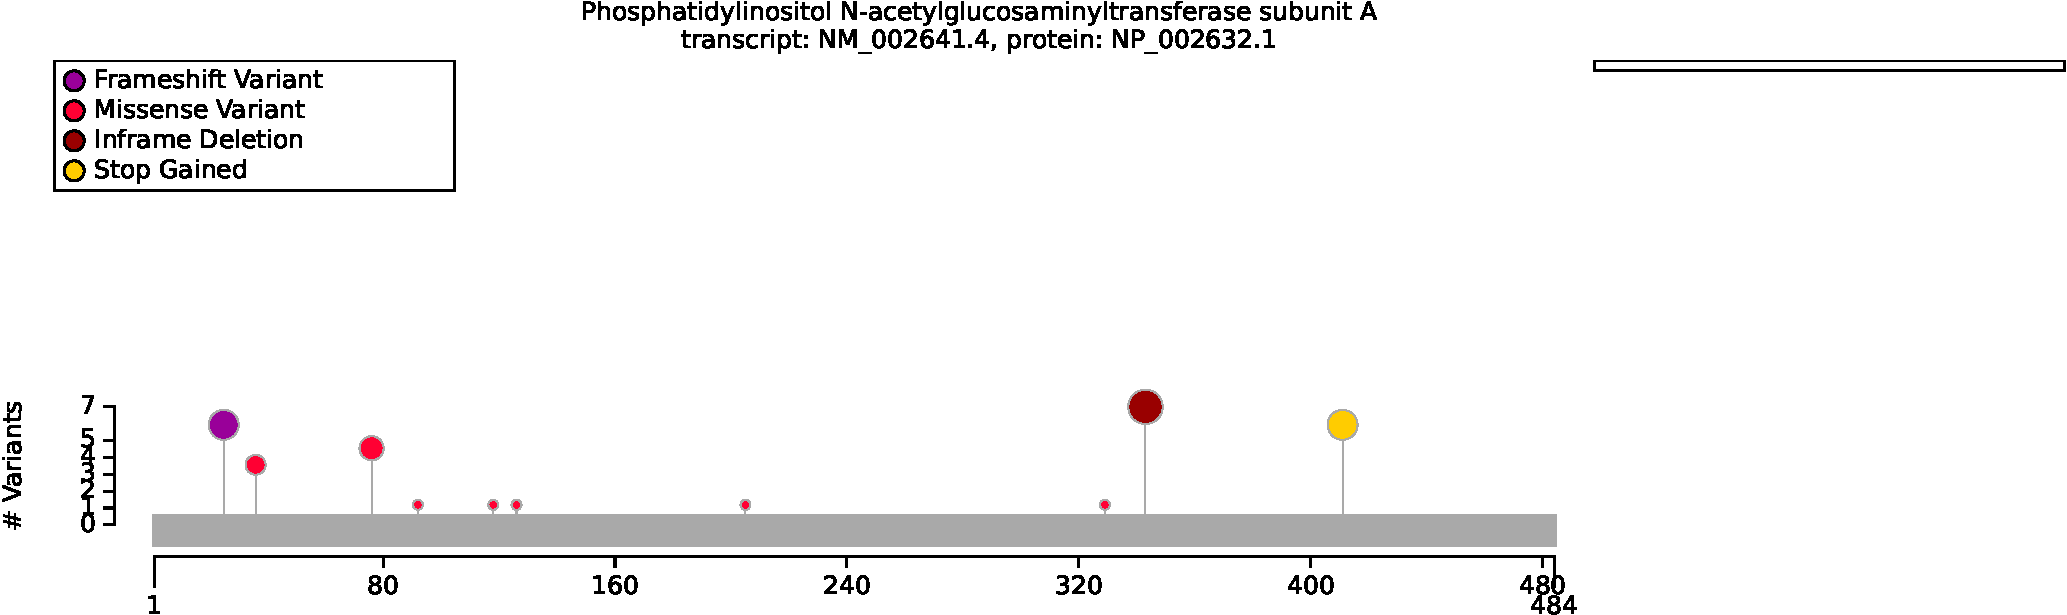
\includegraphics[width=\textwidth]{ img/PIGA_protein_diagram.pdf} 
\captionsetup{justification=raggedright,singlelinecheck=false}
\caption{Distribution of variants in PIGA}
\end{subfigure}

\vspace{2em}

\begin{subfigure}[b]{0.95\textwidth}
\centering
\resizebox{\textwidth}{!}{
\begin{tabular}{llllrr}
\toprule
Genotype (A) & Genotype (B) & total tests performed & significant results\\
\midrule
missense & other & 23 & 0\\
p.Leu344del & other & 20 & 0\\
1-100 & 100+ & 23 & 0\\
\bottomrule
\end{tabular}
}
\captionsetup{justification=raggedright,singlelinecheck=false}
\caption{Fisher Exact Test performed to compare HPO annotation frequency with respect to missense, p.Leu344del, and N-terminal (1-100) and other. }
\end{subfigure}


\vspace{2em}

\caption{The cohort comprised 27 individuals (0 females, 27 males). A total of 188 HPO terms were used to annotate the cohort. Disease diagnoses: Multiple congenital anomalies-hypotonia-seizures syndrome 2 (OMIM:300868) (21 individuals), Neurodevelopmental disorder with epilepsy and hemochromatosis (OMIM:301072) (6 individuals). No statistically significant results identified. A total of 12 unique variant alleles were found in \textit{PIGA} (transcript: \texttt{NM\_002641.4}, protein id: \texttt{NP\_002632.1}).}
\end{figure}
